\let\negmedspace\undefined
\let\negthickspace\undefined
\documentclass[journal]{IEEEtran}
\usepackage[a5paper, margin=10mm, onecolumn]{geometry}
%\usepackage{lmodern} % Ensure lmodern is loaded for pdflatex
\usepackage{tfrupee} % Include tfrupee package

\setlength{\headheight}{1cm} % Set the height of the header box
\setlength{\headsep}{0mm}     % Set the distance between the header box and the top of the text

\usepackage{gvv-book}
\usepackage{gvv}
\usepackage{cite}
\usepackage{amsmath,amssymb,amsfonts,amsthm}
\usepackage{algorithmic}
\usepackage{graphicx}
\usepackage{textcomp}
\usepackage{xcolor}
\usepackage{txfonts}
\usepackage{listings}
\usepackage{enumitem}
\usepackage{mathtools}
\usepackage{gensymb}
\usepackage{comment}
\usepackage[breaklinks=true]{hyperref}
\usepackage{tkz-euclide} 
\usepackage{listings}
% \usepackage{gvv}                                        
\def\inputGnumericTable{}                                 
\usepackage[latin1]{inputenc}                                
\usepackage{color}                                            
\usepackage{array}                                            
\usepackage{longtable}                                       
\usepackage{calc}                                             
\usepackage{multirow}                                         
\usepackage{hhline}                                           
\usepackage{ifthen}                                           
\usepackage{lscape}
\begin{document}

\bibliographystyle{IEEEtran}
\vspace{3cm}




\title{
%	\logo{
GATE - 2007 - EE

\large{EE1030 : Matrix Theory}

Indian Institute of Technology Hyderabad
%	}
}
\author{Satyanarayana Gajjarapu

AI24BTECH11009
}	





\maketitle




\bigskip

\renewcommand{\thefigure}{\theenumi}
\renewcommand{\thetable}{\theenumi}


\section{35 - 51}


\begin{enumerate}
\item The system $\frac{900}{s\brak{s+1}\brak{s+9}}$ is to be compensated such that its gain-crossover frequency becomes same as its uncompensated phase-crossover frequency and provides a $45\degree$ phase margin. To achieve this, one may use
    \begin{enumerate}
        \item a lag compensator that provides an attenuation of 20 dB and a phase lag of $45\degree$ at the frequency of $3\sqrt{3}$ rad/s
        \item a lead compensator that provides an amplification of 20 dB and a phase lead of $45\degree$ at the frequency of 3 rad/s
        \item a lag-lead compensator that provides an amplification of 20 dB and a phase lag of $45\degree$ at the frequency of $\sqrt{3}$ rad/s
        \item a lag-lead compensator that provides an attenuation of 20 dB and a phase lead of $45\degree$ at the frequency of 3 rad/s \\
    \end{enumerate}
\item Consider the discrete-time system shown in the figure where the impulse response of $G\brak{z}$ is $g\brak{0}=0$, $g\brak{1}=g\brak{2}=1$, $g\brak{3}=g\brak{4}=\cdots=0$.
\begin{figure}[h!]
	    \centering
	    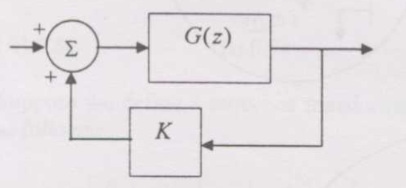
\includegraphics[width=0.7\linewidth]{figs/Q2.png}
     \end{figure}\\
     This system is stable for range of values of $K$
\begin{enumerate}
    \item $\sbrak{-1, \frac{1}{2}}$
    \item $\sbrak{-1, 1}$
    \item $\sbrak{-\frac{1}{2}, 1}$
    \item $\sbrak{-\frac{1}{2}, 2}$ \\
\end{enumerate}
\item A signal $x\brak{t}$ is given by 
\begin{align*}
    x\brak{t} = 
    \begin{cases}
        1, -\frac{T}{4} < t \leq \frac{3T}{4} \\
        -1, \frac{3T}{4} < t \leq \frac{7T}{4} \\
        -x\brak{t + T}
    \end{cases}
\end{align*}
Which among the following gives the fundamental Fourier term of $x\brak{t}$? 
\begin{enumerate}
    \item $\frac{4}{\pi}\cos\brak{\frac{\pi t}{T} - \frac{\pi}{4}}$
    \item $\frac{\pi}{4}\cos\brak{\frac{\pi t}{2T} + \frac{\pi}{4}}$
    \item $\frac{4}{\pi}\sin\brak{\frac{\pi t}{T} - \frac{\pi}{4}}$
    \item $\frac{\pi}{4}\sin\brak{\frac{\pi t}{2T} + \frac{\pi}{4}}$ \\
\end{enumerate}
 \item If the loop gain $K$ of a negative feedback system having a loop transfer function $\frac{K\brak{s+3}}{\brak{s+8}^2}$ is to be adjusted to induce a sustained oscillation then
 \begin{enumerate}
     \item The frequency of this oscillation must be $\frac{4}{\sqrt{3}}$ rad/s
     \item The frequency of this oscillation must be 4 rad/s
     \item The frequency of this oscillation must be 4 or $\frac{4}{\sqrt{3}}$ rad/s
     \item such a $K$ does not exist \\
 \end{enumerate}
\item The system shown in figure below
\begin{figure}[h!]
	    \centering
	    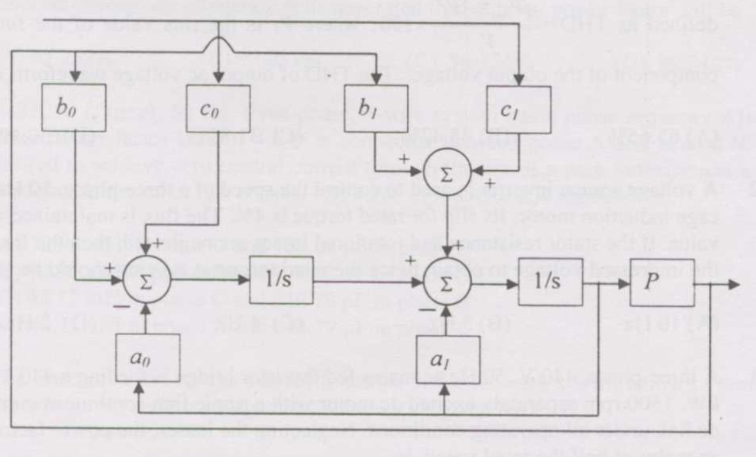
\includegraphics[width=0.7\linewidth]{figs/Q5.1.png}
     \end{figure}\\
can be reduced to the form
\begin{figure}[h!]
	    \centering
	    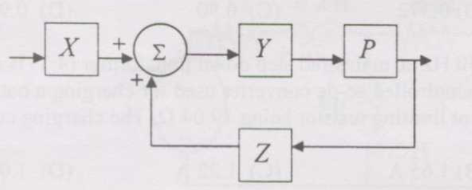
\includegraphics[width=0.5\linewidth]{figs/Q5.2.png}
     \end{figure}\\
with
\begin{enumerate}
    \item $X = c_0s + c_1$, $Y = \frac{1}{\brak{s^2 + a_0s + a_1}}$, $Z = b_0s + b_1$
    \item $X = 1$, $Y = \frac{\brak{c_0s + c_1}}{\brak{s^2 + a_0s + a_1}}$, $Z = b_0s + b_1$
    \item $X = c_1s + c_0$, $Y = \frac{\brak{b_1s + b_0}}{\brak{s^2 + a_1s + a_1}}$, $Z = 1$
    \item $X = c_1s + c_0$, $Y = \frac{1}{\brak{s^2 + a_1s + a_1}}$, $Z = b_1s + b_0$ \\
\end{enumerate}
\item The value of $\ointctrclockwise\limits_{C} \frac{dz}{\brak{1 + z^2}}$ where $C$ is the contour $\abs{z - \frac{i}{2}} = 1$ is
\begin{enumerate}
    \item $2 \pi i$
    \item $\pi$
    \item $\tan^{-1}z$
    \item $\pi i \tan^{-1}z$ \\
\end{enumerate}
\item A single-phase voltage source inverter is controlled in a single pulse-width modulated mode with a pulse width of $150\degree$ in each half cycle. Total harmonic distortion is defined as 
\begin{align*}
    \text{THD} = \frac{\sqrt{V_{rms}^2 - V_1^2}}{V_1} \times 100, 
\end{align*}where $V_1$ is the rms value of the fundamental component of the output voltage. The THD of output ac voltage waveform is
\begin{enumerate}
    \item 65.65\%
    \item 48.42\%
    \item 31.83\%
    \item 30.49\% \\
\end{enumerate}
\item A voltage source inverter is used to control the speed of a three-phase, 50 Hz, squirrel cage induction motor. Its slip for rated torque is 4\%. The flux is maintained at rated value. If the stator resistance and rotational losses are neglected, then the frequency of the impressed voltage to obtain twice the rated torque at starting should be
 \begin{enumerate}
     \item 10 Hz
     \item 5 Hz
     \item 4 Hz
     \item 2 Hz \\
 \end{enumerate}
\item A three-phase, 440 V, 50 Hz ac mains fed thyristor bridge is feeding a 440 V dc, 15 kW, 1500 rpm separately excited dc motor with a ripple free continuous current in the dc link under all operating conditions. Neglecting the losses, the power factor of the ac mains at half the rated speed, is
\begin{enumerate}
     \item 0.354
     \item 0.372
     \item 0.90
     \item 0.955 \\
 \end{enumerate}
\item A single-phase, 230 V, 50 Hz ac mains fed step down transformer \brak{4:1} is supplying power to a half-wave uncontrolled ac-dc converter used for charging a battery (12 V dc) with the series current limiting resistor being 19.04 $\Omega$. The charging current is
\begin{enumerate}
    \item 2.43 A
    \item 1.65 A
    \item 1.22 A
    \item 1.0 A \\
\end{enumerate}
\item A three-phase synchronous motor connected to ac mains is running at full load and unity power factor. If its shaft load is reduced by half, with field current held constant, its new power factor will be
\begin{enumerate}
    \item unity
    \item leading
    \item lagging
    \item dependent on machine parameters \\
\end{enumerate}
\item A 100 kVA, 415 V (line), star-connected synchronous machine generates rated open circuit voltage of 415 V at a field current of 15 A. The short circuit armature current at a field current of 10 A is equal to the rated armature current. The per unit saturated synchronous reactance is
\begin{enumerate}
    \item 1.731
    \item 1.5
    \item 0.666
    \item 0.577 \\
\end{enumerate}
\item A three-phase, three-stack, variable reluctance step motor has 20 poles on each rotor and stator stack. The step angle of this step motor is
\begin{enumerate}
    \item 3\degree
    \item 6\degree
    \item 9\degree
    \item 18\degree \\
\end{enumerate}
\item A single-phase 50 kVA, 250V/500V two winding transformer has an efficiency of 95\% at full load, unity power factor. If it is reconfigured as a 500V/750V autotransformer, its efficiency at its new rated load at unity power factor will be
\begin{enumerate}
   \item 95.752\%
   \item 97.851\%
   \item 98.276\%
   \item 99.241\% \\
\end{enumerate}
\item A 230 V (Phase), 50 Hz, three-phase, 4-wire system has a phase sequence ABC. A unity power-factor load of 4 kW is connected between phase A and neutral N. It is desired to achieve zero neutral current through the use of a pure inductor and a pure capacitor in the other two phases. The value of inductor and capacitor is
\begin{enumerate}
    \item 72.95 mH in phase C and 139.02 $\mu$F in phase B
    \item 72.95 mH in phase B and 139.02 $\mu$F in phase C
    \item 42.12 mH in phase C and 240.79 $\mu$F in phase B
    \item 42.12 mH in phase B and 240.79 $\mu$F in phase C \\
\end{enumerate}
\item The state equation for the current $I_1$ shown in the network below in terms of the voltage $V_x$ and the independent source $V$, is given by
\begin{figure}[h!]
	    \centering
	    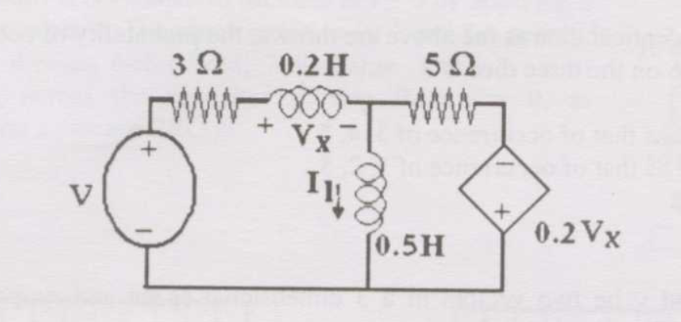
\includegraphics[width=0.7\linewidth]{figs/Q16.png}
     \end{figure}
\begin{enumerate}
    \item $\frac{dI_1}{dt} = -1.4V_x - 3.75I_1 + \frac{5}{4}V$
    \item $\frac{dI_1}{dt} = 1.4V_x - 3.75I_1 - \frac{5}{4}V$
    \item $\frac{dI_1}{dt} = -1.4V_x + 3.75I_1 + \frac{5}{4}V$
    \item $\frac{dI_1}{dt} = -1.4V_x + 3.75I_1 - \frac{5}{4}V$
\end{enumerate}
\item If $u\brak{t}$, $r\brak{t}$ denote the unit step and unit ramp functions respectively and $u\brak{t}*r\brak{t}$ their convolution, then the function $u\brak{t+1}*r\brak{t-2}$ is given by
\begin{enumerate}
    \item $\brak{\frac{1}{2}}\brak{t-1}\brak{t-2}$
    \item $\brak{\frac{1}{2}}\brak{t-1}\brak{t-2}$
    \item $\brak{\frac{1}{2}}\brak{t-1}^2u\brak{t-1}$
    \item none of the above
\end{enumerate}
			 \end{enumerate}
			 \end{document}
 
